\documentclass{article}
\usepackage{graphicx}
\usepackage{amsmath}
\usepackage[a4paper, total={6.4in, 8.2in}]{geometry}

\begin{document}



\part*{High-Speed Atomic Force Microscopy to Reveal the Structural Dynamics of the Amyloid-$\beta$ Aggregation Pathways}
The morphological characteristics and aggregation of Amyloid-$\beta$ in this brain has a considerable influence on the risk of Alzheimer's disease. In recent years, many studies have been conducted to characterize the morphology of Amyloid-$\beta$ using AFM (Atomic Force Microscopy). This assignment aims to characterize Amyloid-$\beta$ fibers from AFM images, in particular by calculating the \textit{mean diameter} and \textit{tortuosity} of these fibers. 

In order to calculate the \textit{mean diameter} $d_m$ of the fibers, a method based on the combination of skeletonization and distance map calculation is proposed and the \textit{tortuosity} $\tau$ is defined as follow:
\begin{equation}
\tau = l_m/l \in [0;1]
\label{eq:tor}
\end{equation}
with $l$ the total length of the fiber and $l_m$ the length of a straight line connecting the two ends of the fiber. The tortuosity of a straight line is thus equals to 1. A good approximation of tortuosity can be obtained by calculating the length of the skeleton $l_s$ for $l$ and the maximum Feret diameter $F_{\max}$ for $l_m$. Equation~\eqref{eq:tor} is then written:
\begin{equation}
\tau = F_{\max} / l_s
\label{eq:tor2}
\end{equation}


\begin{figure}[!h]
\begin{center}
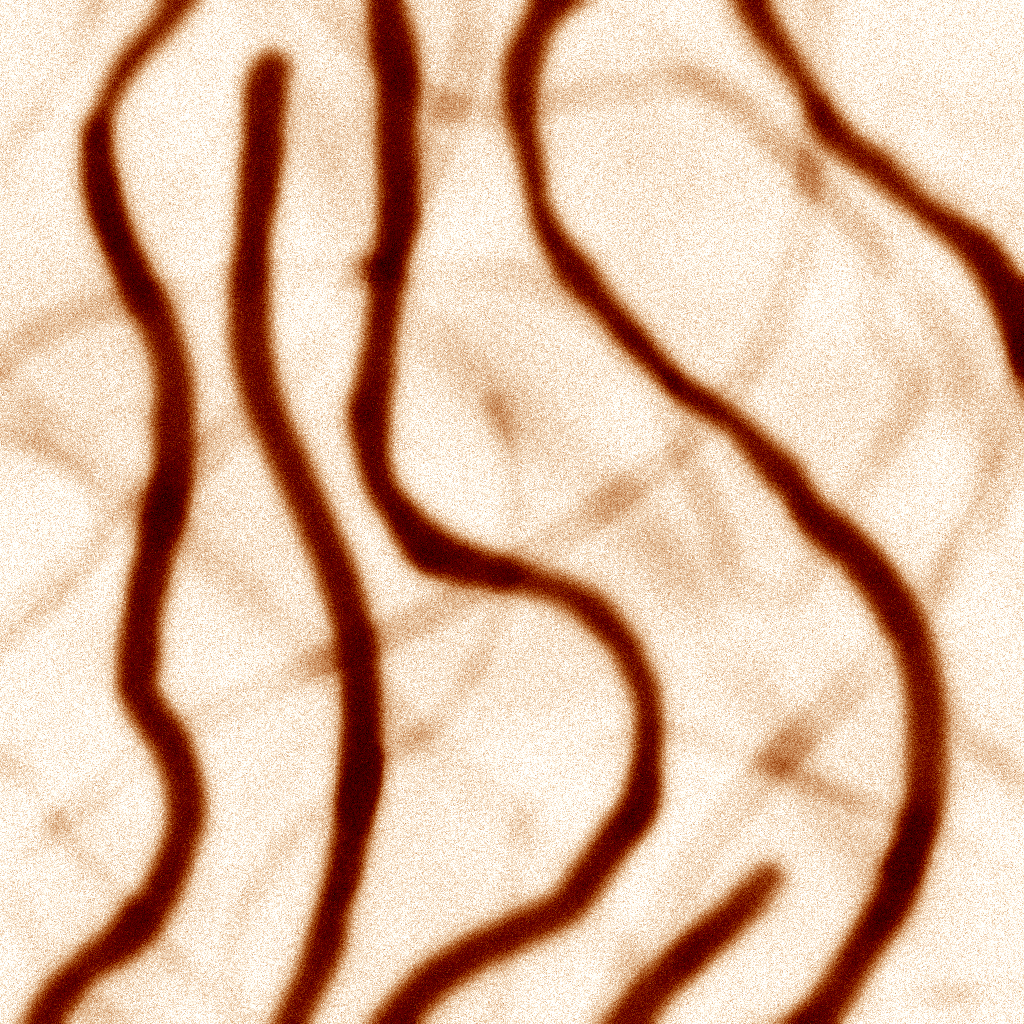
\includegraphics[width=.3\textwidth]{amyloid_b_afm.png}
\qquad
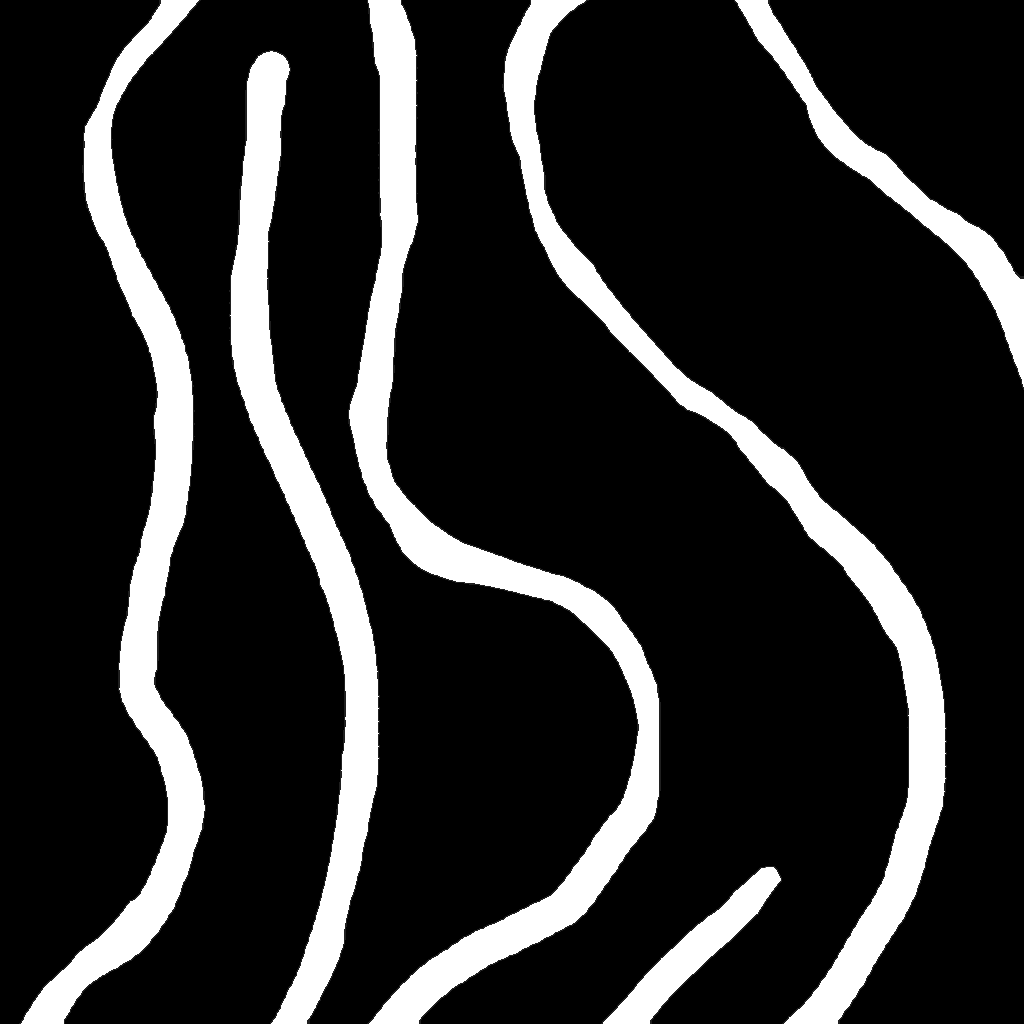
\includegraphics[width=.3\textwidth]{amyloid_b_bw.png}
\label{Fig:AFM_and_BW}
\caption{AFM image of Amyloid-$\beta$ fibers and corresponding segmented binary image.}
\end{center}
\end{figure}

\paragraph*{\textbf{Instructions}}
\begin{itemize}
\item[•] The student has at his disposal a AFM image named \texttt{amyloid\_b\_afm.png} and a corresponding binarized image named \texttt{amyloid\_b\_bw.png}.
\item[•] If the student is having difficulty with the image processing and segmentation portion of the assignment, he or she can use the proposed binary image to answer the following questions.
\end{itemize}


\section*{Question 1 (5 points)}
Propose a method and code a function that turns the AFM image into a binary image in order to isolate every Amyloid-$\beta$ fiber visible on the image.

\section*{Question 2 (2 points)}
Propose a method and code a function that returns the number of fibers. The functions \texttt{skimage.measure.label} (Python) or \texttt{bwlabel} (MATLAB) could be found useful.

\section*{Question 3 (2 points)}
For each fiber, compute the corresponding skeleton. The functions \texttt{skimage.morphology.skeletonize} (Python) or \texttt{bwskel} (MATLAB) could be found useful.

\section*{Question 4 (2 points)}
For each fiber, compute the corresponding distance map. The functions \texttt{scipy.ndimage.distance\_transform\_edt} (Python) or \texttt{bwdist} (MATLAB) could be found useful.

\section*{Question 5 (5 points)}
Propose a method to calculate the \textit{mean diameter} of each fiber. You can use the skeletons and the distance maps previously computed. You should find a value of about 30 pixels.

\section*{Question 6 (4 points)}
Propose a method to calculate the \textit{tortuosity} of each fiber.






\section*{Appendix}
Figure~\ref{Fig:BWLABEL} shows an example of the application of the \texttt{skimage.measure.label} and \texttt{bwlabel} functions to a binary image.
\begin{figure}[!h]
\begin{center}
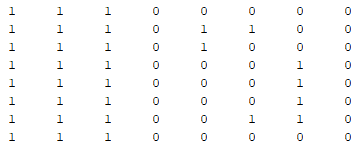
\includegraphics[width=.45\textwidth]{BW.png}
\qquad
\vline
\qquad
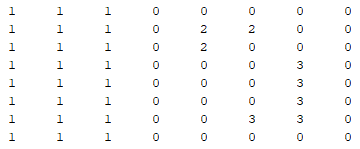
\includegraphics[width=.45\textwidth]{LABEL.png}
\label{Fig:BWLABEL}
\caption{Left: Digital representation of a binary image. Right: Output provided by the \texttt{bwlabel} or \texttt{skimage.measure.label} functions applied to the same binary image.}
\end{center}
\end{figure}

Figure~\ref{Fig:SKEL} shows an example of the application of the \texttt{skimage.measure.label} and \texttt{bwlabel} functions to a binary image.
\begin{figure}[!h]
\begin{center}
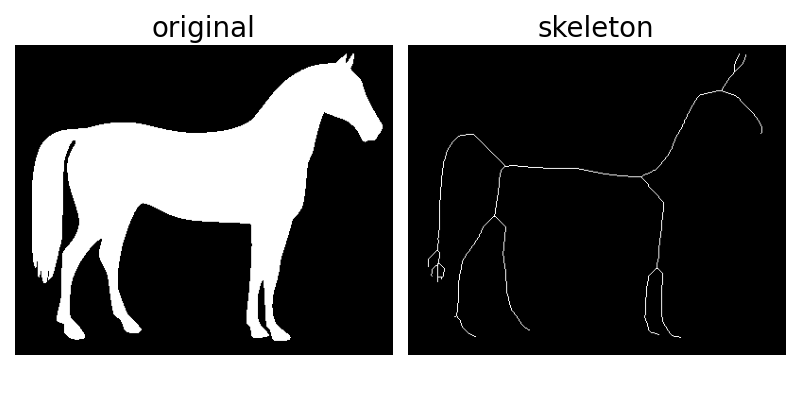
\includegraphics[width=.90\textwidth]{sphx_glr_plot_skeleton_001.png}
\label{Fig:SKEL}
\caption{Left: Digital representation of a binary image. Right: Output provided by the \texttt{bwskel} or \texttt{skimage.morphology.skeletonize} functions applied to the same binary image.}
\end{center}
\end{figure}

Figure~\ref{Fig:BWD} shows an example of the application of the \texttt{scipy.ndimage.distance\_transform\_edt} and \texttt{bwdist} functions to a binary image.
\begin{figure}[!h]
\begin{center}
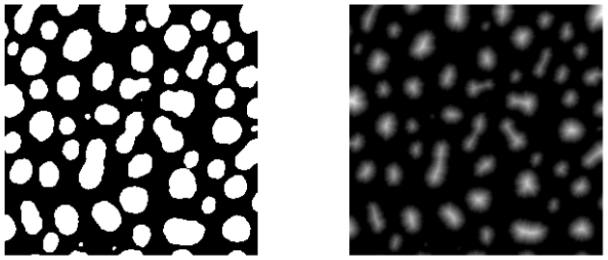
\includegraphics[width=.90\textwidth]{BWD.png}
\label{Fig:BWD}
\caption{Left: Digital representation of a binary image. Right: Output provided by the \texttt{bwdist} or \texttt{scipy.ndimage.distance\_transform\_edt} functions applied to the same binary image.}
\end{center}
\end{figure}




\end{document}
